%Typeset using XeLaTeX

\documentclass[10pt,a4paper]{book}
\usepackage{mathtools,amssymb,amsthm}
%\usepackage{phonetic}
\usepackage{fancyhdr}
\usepackage[pass]{geometry}
\usepackage{fontspec}
%\usepackage{xunicode}
%\usepackage{xltxtra}
%\usepackage{xgreek}
\setmainfont[Mapping=TeX-text]{Times New Roman}
\usepackage{hyperref}
%\usepackage{color}
\usepackage[Glenn]{fncychap}
\ChNameVar{\bfseries\Large}
%\usepackage{tabularx}
%\usepackage[normalem]{ulem}

%\usepackage{tikz}
\usepackage{enumerate}
\usepackage{natbib}

\renewcommand{\maketitle}{
	\begin{titlepage}
		\newgeometry{left=4cm, top=2.3cm, bottom=2.3cm}
		\hbox{\mbox{\hspace{-1.3cm}}
			\vrule depth 0.98\textheight
			\mbox{\hspace{1cm}}
			\vtop{
				\vspace{2cm}
				\begin{flushleft}
					\huge{\bf Profit Games in Heterogeneous 2-link Parallel Networks\\}
					\vskip3cm
					\Large  Thomas Pappas\\
					AL1.18.0011\\
					\vskip3cm
					\begin{minipage}{7.5cm}
						\begin{flushleft}
							\normalsize {\it {\bf Examination committee:}\\
								Dimitris Fotakis, School of Electrical and Computer Engineering, National Technical University of Athens.\\
								Professor's name, Department or School, Institution.\\
								Professor's name, Department or School, Institution.}
						\end{flushleft}
					\end{minipage}
					\hskip0.5cm
					\begin{minipage}{6cm}
						\begin{flushleft}
							\normalsize {\it {\bf Supervisor:}\\
								Dimitris Fotakis, Professor, \\ School of Electrical and Computer Engineering,\\
								National Technical University of Athens.\\
							}
						\end{flushleft}
					\end{minipage}
				\end{flushleft}
				\vskip6cm
				\hskip4.5cm
				\begin{minipage}{5cm}
					\begin{center}
						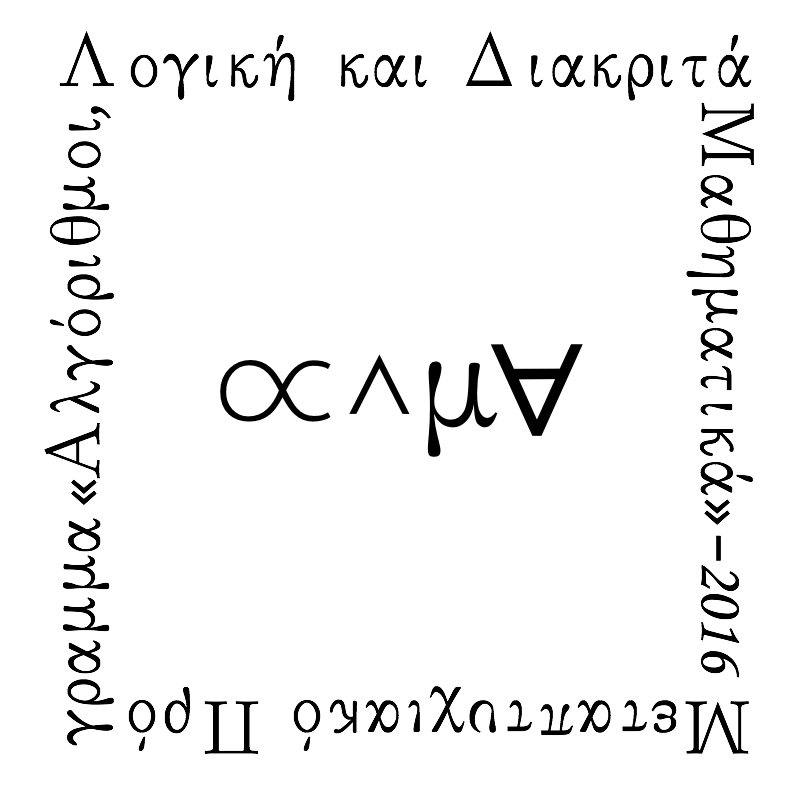
\includegraphics[width=0.8\textwidth]{alma.png}
					\end{center}
		\end{minipage}}}
	\end{titlepage}
}

% Commands for wrapping properly common expressions.
\newcommand{\indeq}[1]{\stackrel{\text{#1}}{=}}
\newcommand{\RightarrowArg}[1]{\stackrel{#1}{\Longrightarrow}}
\newcommand{\LeftrightarrowArg}[1]{\stackrel{#1}{\Leftrightarrow}}
\newcommand{\NE}{\mathrm{N.E.}}
\newcommand{\as}{\mathrm{\alpha_s}}
\newcommand{\R}{\mathbb{R}}
\DeclareMathOperator*{\argmax}{arg\,max}
% \newcommand{\Exp}{\mathrm{Exp}}
% \newcommand{\Expect}{{\rm I\kern-.3em E}}

% Theorem structures.
\theoremstyle{definition}
\newtheorem{ex}{}[section]
\newtheorem{definition}{Definition}[chapter]
\newtheorem{theorem}[definition]{Theorem}
\newtheorem{lemma}[definition]{Lemma}
\newtheorem{corollary}[definition]{Corollary}
\theoremstyle{comment}
\newtheorem{example}[definition]{Example}
\newtheorem{claim}[definition]{Claim}

\fancyhead[LO]{\slshape \leftmark}
\fancyhead[RE]{\slshape \rightmark}
\fancyhead[LE]{}
\fancyhead[RO]{}
\fancyfoot[LO,RE]{\tiny{\it}}

% Main document
\begin{document}

\maketitle
\clearpage


\thispagestyle{empty}
\null
\clearpage

\restoregeometry

\thispagestyle{empty}
\pagenumbering{gobble}
\chapter*{Abstract}
In this masters thesis we study a $2$-level optimisation problem where, on a $2$-link network from a source $s$ to a target $t$, a unit of flow wants to move from $s$ to $t$ using the link with the lowest cost, while the two link owners compete for profit by assigning tolls to links and thus creating a toll congestion game.
We examine only affine latencies for the links.
In addition, each flow player responds to tolls in a heterogeneous way, i.e. each flow player $p$ has a different money-time sensitivity value, which is described by a distribution function $\alpha(p)$.
First we present some basic definitions and properties of profit homogeneous games.
Using them as base, we examine cases of fixed and step distribution functions, where for the latter we present strict conditions for the existence or not of a Nash Equilibrium.
We then introduce a new term, the split function $\as(t)$, defined as the time-money sensitivity value for which the $2$ link costs are equal for a given set of tolls $t$. With the help of $\as$ we will describe and prove some properties of the heterogeneous games for continuous distribution functions.
In our main result, we generalise the conditions necessary for the existence of a Nash Equilibrium in the profit game between the toll owners, and finally we discuss some extensions to $n$-link parallel networks.
\clearpage

\thispagestyle{empty}
\null
\clearpage

\thispagestyle{empty}
\pagenumbering{gobble}
\chapter*{Συνοψη}
Σε αυτή τη διπλωματική μεταπτυχιακού μελετάμε ένα πρόβλημα βελτιστοποίησης $2$ επιπέδων, όπου σε ένα δίκτυο με $2$ ακμές από μια πηγή $s$ σε ένα στόχο $t$, μια μονάδα ροής θέλει να μετακινηθεί από το $s$ στο $t$ χρησιμοποιώντας την ακμή με το χαμηλότερο κόστος, ενώ οι δύο ιδιοκτήτες των ακμών ανταγωνίζονται για κέρδος βάζοντας δίοδια στις ακμές και δημιουργώντας έτσι ένα παίγνιο συμφόρησης με διόδια.
Εξετάζουμε μόνο αφινικές καθυστερήσεις για τις ακμές.
Επιπλέον, ο κάθε παίκτης ροής αντιδρά στα διόδια με ετερογενή τρόπο, δηλ. ο κάθε παίκτης ροής $p$ έχει διαφορετική τιμή ευαισθησίας χρόνου-χρήματος, η οποία περιγράφεται από μια συνάρτηση κατανομής $\alpha(p)$.
Πρώτα παρουσιάζουμε κάποιους βασικούς ορισμούς και ιδιότητες των ομογενών παιγνίων κέρδους. Mε αυτά ως βάση, εξετάζουμε περιπτώσεις σταθερών και βηματικών συναρτήσεων κατανομής, όπου για το τελευταίο παρουσιάζουμε αυστηρές συνθήκες για την ύπαρξη ή μη σημείου ισορροπίας Nash.
Μετά εισαγάγουμε έναν νέο όρο, τη συνάρτηση διαχωρισμού $\as(t)$, ορισμένη ως η τιμή ευαισθησίας χρόνου-χρήματος για την οποία τα κόστη των $2$ ακμών είναι ίσα για ένα δοσμένο σετ διοδίων $t$.
Με τη βοήθεια της $\as$ θα περιγράψουμε και θα αποδείξουμε μερικές ιδιότητες των ετερογενών παιγνίων με συνεχή συνάρτηση κατανομής.
Στο κύριο αποτέλεσμά μας, γενικοποιούμε τις συνθήκες που είναι απαραίτητες για την ύπαρξη ισορροπίας Nash στο παίγνιο κέρδους μεταξύ των ιδιοκτητών των ακμών, και τελικώς συζητάμε κάποιες επεκτάσεις για δίκτυα με $n$ ακμές.
\clearpage

\thispagestyle{empty}
\null
\clearpage


\clearpage
\thispagestyle{empty}

\pagestyle{fancy}

\pagenumbering{roman}
\tableofcontents
\clearpage

\thispagestyle{empty}
\null
\clearpage

\pagenumbering{arabic}


\chapter{Introduction}

In this thesis we study a three level optimisation problem.
On the basis there is a 2-node $(s, t)$, 2-link $s-t$ network, each link with a non-decreasing latency function that defines how the traffic increases as more players flow into that link.
On the first level a flow $[0, 1]$ wants to move from $s$ to $t$ and experience the minimum latency (traffic).
On the second level, the links might also have tolls which impose an additional cost to the flow players, plus in our case (heterogeneous users) each player has a different money-time trade-off and thus see the link costs differently.
Finally on the third level (are the levels really that way?), the tolls are owned by players who profit on the flow that uses that link and compete to maximise it.

We know from Cole et al. \cite{10.1145/780542.780618} that regardless of the distribution function $a$ or the latency functions (as long as they are non-decreasing) a $\NE$ always exists.
In that $\NE$ the users are split with the money-sensitive ones on the link with the lower toll and the time-sensitive ones on the higher toll one, each one seeing their link as either lower or equal cost with the other (while they all see traffic equally).

We introduce a new term $\as=\frac{l_1(x)-l_2(1-x)}{t_2-t_1}$ which is the $a(p)$ value of a user $p$ which sees the link costs equally.


\chapter{Related Work}
TODO


\chapter{Preliminaries}

A 2-link $s-t$ parallel network is a graph with a source node $s$, a destination node $t$ and $2$ edges connecting $s$ to $t$.
Each link is associated with a latency function $l_1, l_2$
[TODO: Add figure]
A flow of infinitesimal users totaling up to a flow of $[0, 1]$ wishes to move from $s$ to $t$ through the link with the lowest cost.


\chapter{2-link parallel networks}

We start with the simple case of 2-link parallel networks.
[TODO: Add figure]
In this simple setup a user of the flow 

\section{Time-money sensitivity split}

Consider a 2-link parallel network with latency functions $l_1(x), l_2(x)$ and tolls $t=(t_1, t_2)$ assigned to them.
Without loss of generality we assume $t_1 > t_2$ which in turn means that for the resulting equilibrium flow $x = (x_1(t), x_2(t))$ it holds that $l_1(x_1(t)) < l_2(x_2(t))$.
This equilibrium is guaranteed to exist according to Harks et al. \cite{Harks_2019}.
For the 2 edges of the game we introduce the term time-money sensitivity split $\as(t)$ as the value for which if any player $p$ has $\alpha(p)=\as(t)$ then that player sees the $2$ edge total latencies as equal.
More specifically, $\as(t)$ is the value of the distribution function $\alpha$ for which it holds
\[l_1(x_1(t)) + \as(t) t_1 = l_2(x_2(t)) + \as(t) t_2\]
Solving for $\as$ we get
\[\as(t) = \frac{l_2(x_2(t)) - l_1(x_1(t))}{t_1 - t_2}\]
\\
Before we get into a more formal definition and description of $\as$, it'd help to first discuss the nature of the split that $\as$ captures.
Regardless of whether there exists a player $p$ such that $\alpha(p) = \as(t)$, it still holds that
\begin{itemize}
	\item if $\alpha(p) < \as$ then $l_1(x_1(t)) + \alpha(p) t_1 < l_2(x_2(t)) + \alpha(p) t_2$, thus $p$ is on edge $1$
	\item if $\alpha(p) > \as$ then $l_1(x_1(t)) + \alpha(p) t_1 > l_2(x_2(t)) + \alpha(p) t_2$, thus $p$ is on edge $2$
	\item if $\alpha(p) = \as$ then $l_1(x_1(t)) + \alpha(p) t_1 = l_2(x_2(t)) + \alpha(p) t_2$, thus $p$ is either on edge $1$ or $2$
\end{itemize}
Remember that we have assumed that $t_1 > t_2 \Rightarrow l_1(x_1(t)) < l_2(x_2(t))$.
Therefore the flow passing through the faster edge $1$ is contained with players where $\alpha(p) \le \as(t)$, while the flow in the cheaper edge $2$ is contained with players where $\alpha(p) \ge \as(t)$.
Since the players are sorted in increasing order according to $\alpha$, it helps to view the players in the first case as the "lower" part of the split and respectively the players in the second case as the "higher" part of the split.
[TODO: Alternative splits: rushed-relaxed, rich-poor]
Table \autoref{table:split_summary} provides of a summary for each part of the split

\begin{table}[h!]
	\centering
	\caption{Summary of properties for the sensitivity split.}
	\begin{tabular}{| c || c | c |}
		\hline
		& $\alpha(p) \le \as(t)$ & $\alpha(p) \ge \as(t)$ \\ \hline
		sensitivity & time $\ge$ money & time $\le$ money \\ \hline
		latency & lower $(l_2)$ & higher $(l_1)$ \\ \hline
		toll & higher $(t_1)$ & lower $(t_2)$ \\ \hline
		edge & low-latency, high-toll $(1)$ & high-latency, low-toll $(2)$ \\ \hline
		$t_1 - t_2$ & lower & higher \\ \hline
		split & lower & higher \\ \hline
	\end{tabular}
	\label{table:split_summary}
\end{table}

Finally to acknowledge that we have arbitrarily handled any players with $\alpha(p) = \as(t)$.
Those players, if any, even though they see both edges with equal total cost, in the optimal flow $x$ they have settled in either edge $1$ or $2$.
We investigate more in depth the relation of $\as$ to the flow in [TODO: add ref].
\\[12pt]
We can now formally define $\as$ and prove some of its properties.
\begin{definition}
	Given a 2-link parallel heterogeneous game with latency functions $l_1, l_2$, we define the time-money sensitivity split function $\as: \R^2_+ \rightarrow (0, +\infty)$ where for given tolls $t = (t_1, t_2)$
	\[\as(t) = \frac{l_2(x_2(t)) - l_1(x_1(t))}{t_1 - t_2}\]
\end{definition}
The function is well defined since the given tolls $t$ result in a single optimal flow $x(t) = (x_1(t), x_2(t))$ \cite{Harks_2019}.

We start with some basic properties.
\begin{lemma}
	\label{lemma:split_basic}
	Given a 2-link parallel heterogeneous game with distribution function $\alpha$ and time-money sensitivity split function $\as$, the following hold:
	\begin{enumerate}[(i)]
		\item $\as(t) > 0$
		\item if $x_1(t), x_2(t) > 0$ then $\as(t) \in [\alpha(0), \alpha(1)]$
		\item if $0 < l_1(x_1(t)) < l_2(x_2(t))$ then $\alpha(x_1(t)) \le \as(t) \le \alpha(x_1(t) + \epsilon), \forall \epsilon > 0$ arbitrarily small
	\end{enumerate}
\end{lemma}

\begin{proof}
	$ $ % Just to make a line break after "Proof".
	\begin{enumerate}[(i)]
		\item Obviously $\as(t) \ne 0$ since $\as(t) = 0 \Rightarrow l_1(x_1(t)) = l_2(x_2(t))$ which is impossible in a heterogeneous setup.
		Then we only need to notice that $l_1(x_1(t)) < l_2(x_2(t)) \iff t_1 > t_2$ and we get $\as(t) > 0$ from definition.
		\item Since $x_1(t), x_2(t) > 0$ then $\exists p_1, p_2 \in [0, 1]$ each on a different edge, for which we assume w.l.o.g. that $\alpha(p_1) \le \alpha(p_2)$.
		It holds that $\alpha(p_1) \le \as(t) \le \alpha(p_2)$ so with $\alpha$ being non-decreasing it follows
		\[\alpha(0) \le \alpha(p_1) \le \as(t) \le \alpha(p_2) \le \alpha(1) \Rightarrow \as(t) \in [\alpha(0), \alpha(1)]\]
		\item We know that $x_1(t) < x_2(t)$ means that edge 1 has the lower split.
		Therefore we have
		\[\alpha(p) \le \as(t), \forall p \in [0, x_1(t)] \Rightarrow \alpha(x_1(t)) \le \as(t)\]
		Likewise for edge 2 we have
		\[\as(t) \le \alpha(p), \forall p \in (x_1(t), 1] \Rightarrow \as(t) \le \alpha(x_1(t) + \epsilon), \forall \epsilon \in (0, 1 - x_1(t))\]
	\end{enumerate}
\end{proof}

The next lemma will help us describe how $\as(t)$ is changing in relation to toll difference (and in extend to latency difference).
\begin{lemma}
	Given a 2-link parallel heterogeneous game with time-money sensitivity split function $\as$ and tolls $t, t^\prime$ such that $\frac{t_1 - t_2}{t_1^\prime - t_2^\prime} > 0$, the following hold:
	\begin{enumerate}[(i)]
		\item $\as(t) \ge \as(t^\prime)$ iff $\frac{t_1 - t_2}{t_1^\prime - t_2^\prime} \le 1$
		\item $\as(t) \le \as(t^\prime)$ iff $\frac{t_1 - t_2}{t_1^\prime - t_2^\prime} \ge 1$
	\end{enumerate}
\end{lemma}

\begin{proof}
	Before we get into the propositions, notice that the condition
	\begin{equation}
		\frac{t_1 - t_2}{t_1^\prime - t_2^\prime} > 0
		\label{eq:split_property_cond_tolls_0}
	\end{equation}
	ensures that the two tolls provide splits with same edges in their respective lower and higher sections.
	We show this for $t_1 > t_2$ and likewise it also holds for $t_1 < t_2$.
	\[t_1 > t_2 \Leftrightarrow t_1 - t_2 > 0 \LeftrightarrowArg{(\ref{eq:split_property_cond_tolls_0})} t_1^\prime - t_2^\prime > 0 \Leftrightarrow t_1^\prime > t_2^\prime\]
	%Also note that this property extends to the latencies, giving us
	%\begin{equation}
	%	\frac{l_1(x_1(t)) - l_2(x_2(t))}{l_1(x_1^\prime(t)) - l_2(x_2^\prime(t))} > 0
	%	\label{eq:split_property_cond_latencies_0}
	%\end{equation}
	Now moving on to the prepositions, we focus on proving $(i)$ in the right-to-left direction; then the same steps can be followed backwards to prove left-to-right.
	Finally proving $(ii)$ will be much easier as there are many steps symmetric to the ones for $(i)$.
	
	\paragraph{$(i)$}
	Begin by noticing that $\frac{t_1 - t_2}{t_1^\prime - t_2^\prime} \le 1 \Leftrightarrow |t_1 - t_2| \le |t_1^\prime - t_2^\prime|$ (opposite direction is ensured by $(\ref{eq:split_property_cond_tolls_0})$), i.e. the toll difference is increasing.
	Assume w.l.o.g. that $x_1 < x_2$.
	
	If $x_1(t) = 0$ then
	\[\as(t) = \frac{l_2(1)}{t_2 - t_1}, \as(t^\prime) = \frac{l_2(1)}{t_2^\prime - t_1^\prime}\] 
	so obviously $t_2 - t_1 \le t_2^\prime - t_1^\prime \Rightarrow \as(t) \ge \as(t^\prime)$.
	
	If $x_1(t) > 0$ then we know [TODO: do we?] that the latency difference might also increase, with flow from the lower latency edge, if any, moving towards the slower one, i.e. $x_1(t) \ge x_1(t^\prime)$.
	%\[|t_1 - t_2| \le |t_1^\prime - t_2^\prime| \Leftrightarrow |l_1(x_1(t)) - l_2(x_2(t))| \le |l_1(x_1(t^\prime)) - l_2(x_2(t^\prime))|\]
	%\begin{equation}
	%	|l_1(x_1(t)) - l_2(x_2(t))| \le |l_1(x_1(t^\prime)) - l_2(x_2(t^\prime))| \LeftrightarrowArg{(\ref{eq:split_property_cond_latencies_0})} \frac{l_1(x_1(t)) - l_2(x_2(t))}{|l_1(x_1(t^\prime)) - l_2(x_2(t^\prime))|} \le 1
	%	\label{eq:split_property_cond_latencies_1}
	%\end{equation}
	If no flow moves then we can easily show that $\as(t) \ge \as(t^\prime)$ similarly to the case with $x_1(t) = 0$.
	Otherwise we have $x_1(t) > x_1(t^\prime) \Rightarrow \exists \epsilon > 0: x_1(t) = x_1(t^\prime) + \epsilon$ and by carefully applying property $\ref{lemma:split_basic}(ii)$ we get
	\[\as(t^\prime) \le \alpha(x_1(t^\prime) + \epsilon) = \alpha(x_1(t)) \le \as(t)\]
	
	\paragraph{$(ii)$}
	Symmetrically to $(i)$ in this case the toll difference is decreasing, and therefore flow from the higher latency edge will move towards the lower one, i.e. $x_1(t) \le x_1(t^\prime)$ (assuming again $x_1 < x_2$).
	With a similar argument we then get $\as(t) \le \as(t^\prime)$.
\end{proof}

The next lemma gives us some insight of the behavior of $\as(t)$ around its edge values.
\begin{lemma}
	\label{lemma:split_bounds}
	Given a 2-link parallel heterogeneous game with distribution function $\alpha$ and time-money sensitivity split function $\as$, the following hold:
	\begin{enumerate}[(i)]
		\item if $\alpha(0) > 0$ then $\as(t) < \alpha(0) \Rightarrow x(t) = (0, 1)$ or $(1, 0)$
		\item if $x_1(0), x_2(0) > 0$ and $\alpha(0) = 0$ with $0$ an accumulation point, then $x_1(t), x_2(t) > 0, \forall t \in \R_+^2$
		\item $\lim_{|t_1 - t_2| \rightarrow +\infty}\as(t) = 0$
		\item $\lim_{t_1 - t_2 \rightarrow 0^-} \as(t) = \alpha(x_1), \lim_{t_1 - t_2 \rightarrow 0^+} \as(t) = \alpha(x_2)$, where ($x_1, x_2)$ the optimal flow under no tolls
	\end{enumerate}
\end{lemma}

\begin{proof}
	$ $
	\begin{enumerate}[(i)]
		\item Direct consequence from the fact that all players $p$ with $\as(t) < \alpha(p)$ are in the low latency edge.
		\item Since $\alpha(0) = 0$ and $0$ an accumulation point, then $\forall \delta > 0 \exists \epsilon > 0: p < \epsilon \Rightarrow \alpha(p) < \delta$.
		Therefore $\forall t \in \R_+^2$ if $\delta = \as(t)$ then $\exists \epsilon > 0: p < \epsilon \Rightarrow \alpha(p) < \as(t)$, which means that the lower latency edge will always have flow some $\epsilon > 0$, and therefore $x_1(t), x_2(t) > 0$.
		\item We only need to notice that $|l_1(x_1(t)) - l_2(x_2(t))| \le \max\{l_1(1), l_2(1)\} = L$ and we find
		\[\lim_{|t_1 - t_2| \rightarrow +\infty}\as(t) = \lim_{|t_1 - t_2| \rightarrow +\infty}\frac{|l_1(x_1(t)) - l_2(x_2(t))|}{|t_1 - t_2|} \le \lim_{|t_1 - t_2| \rightarrow +\infty}\frac{L}{|t_1 - t_2|} = 0\]
		and since $\as(t) > 0$ we get $\lim_{|t_1 - t_2| \rightarrow +\infty}\as(t) = 0$.
		\item As $|t_1 - t_2| \rightarrow 0$ then also $|l_1(x_1(t)) - l_2(x_2(t))| \rightarrow 0$ as the game approaches the homogeneous case.
		Then flow on the low latency edge will define the limit of $\as(t)$.
			\begin{itemize}
				\item For $t_1 > t_2$ we get lower latency edge $1$ with flow $x_1(t) \rightarrow x_1$ and therefore
				\[\lim_{t_1 - t_2 \rightarrow 0^-} \as(t) = \alpha(x_1)\]
				\item For $t_1 < t_2$ we get lower latency edge $2$ with flow $x_2(t) \rightarrow x_2$ and therefore
				\[\lim_{t_1 - t_2 \rightarrow 0^+} \as(t) = \alpha(x_2)\]
			\end{itemize}
	\end{enumerate}
\end{proof}

From the above lemma we can also observe the following

\begin{corollary}
	Given a 2-link parallel heterogeneous game with distribution function $\alpha$ and time-money sensitivity split function $\as$ and $x = (x_1, x_2)$ the optimal flow in the game without tolls, then $\as(t) \le \max\{\alpha(x_1), \alpha(x_2)\}$.
\end{corollary}

This corollary hints that all values of $\alpha$ above $\max\{x_1, x_2\}$ are irrelevant to the game.
This will become more obvious later when calculating best responses as those values will never be used.
[TODO: Maybe put this in its own Lemma and prove it?]

\section{Profit maximisation and distribution function}

In this section we will examine how different distribution functions $\alpha$ can affect the profit maximisation game between the toll owners.
[TODO: add framework for examining games]
We will restrict our analysis on distribution functions such that $\alpha(0) > 0$, the reason being that we want to avoid two instances.
The first is to ensure that $\alpha(p) > 0$ when $p > 0$, while the second is that $0$ is not an accumulation point.
[TODO: maybe mention \cite{10.1145/780542.780618} where they also take the first restriction as it creates games with no optimal tolls]
The following two examples demonstrate the issues that might occur if these restrictions are not met.

\begin{example}
	Consider a $2$-link parallel network pricing game with distribution function $\alpha$ for which it does not hold that $\alpha(p) > 0$ when $p > 0$.
\end{example}

The property not holding for $\alpha$ means that $\exists x_\epsilon > 0 : \alpha(x_\epsilon) = 0 \forall p < x_\epsilon$.
That $x_\epsilon$ flow will completely neglect the tolls and play the congestion game only considering the flow latency, therefore they will always select the fastest edge regardless of the toll price.
This in turn means that any toll owner can exploit it and set their toll to an arbitrary high value $T$ which will force all players with $\alpha(p) > 0$ to leave, thus making their own edge the fastest one.
Even if the edge has a latency function with a high increasing rate, there will be at least a small flow $x_{\epsilon^\prime} \le x_\epsilon$ on that edge.
Therefore the owner can achieve any arbitrary profit $P$ by setting their toll price as $T + P/\epsilon$.
Since both player have that strategy available, we conclude that no equilibrium exists in the pricing game.

\begin{example}
	\label{example:a_0_ap}
	Consider a $2$-link parallel network pricing game with $l_1(x) = x, l_2(x) = 2x$ and distribution function $\alpha(p) = p$.
\end{example}

Notice that the condition $\alpha(p) > 0$ when $p > 0$ holds for this example.
However in this case $0$ is an accumulation point, and by Lemma $\ref{lemma:split_bounds}(ii)$ it follows $x_1(t), x_2(t) > 0, \forall t \in \R_+^2$.
Then Lemma $\ref{lemma:split_basic}$ entails that, assuming $t_1 > t_2$, $\alpha(x_1(t)) \le \as(t) \le \alpha(x_1(t) + \epsilon), \forall \epsilon > 0$ arbitrarily small, and since in this example $\alpha$ is onto, then $\as(t) = \alpha(x_1(t))$.

We will calculate $B_i(t_{-i})$ by calculating $x_i(t)$ and then finding $\argmax \Pi_i(t)$.
Note that since we always have $x_1(t), x_2(t) > 0$ we don't need to take cases where the flow is on one edge.
For tolls $t = (t_1, t_2)$ and respective optimal flow $x = (x_1(t), x_2(t))$ we take the following cases.

\paragraph{If $t_1 > t_2$}
then $x_1$ is the low-latency flow and thus $\as(t) = \alpha(x_1(t)) = x_1(t)$.
We therefore get
\begin{align}
	l_1(x_1(t)) + \as(t) t_1 &= l_2(x_2(t)) + \as(t) t_2 &\Rightarrow \notag \\
	x_1(t) + x_1(t) t_1 &= 2 (1 - x_1(t)) + x_1(t) t_2 &\Rightarrow \notag \\
	x_1(t) &= \frac{2}{3 + t_1 - t_2} \label{eq:ex2_x1_1}
\end{align}
\[
	B_1^>(t_2) = \argmax_{t_2 < t_1} x_1(t) t_1 \indeq{(\ref{eq:ex2_x1_1})} \argmax_{t_2 < t_1} \frac{2 t_1}{3 + t_1 - t_2} = \argmax_{t_2 < t_1} \frac{2}{1 + \frac{3 - t_2}{t_1}} =
		\begin{cases}
			+\infty, & t_2 < 3 \\
			\textrm{undefined}, & t_2 = 3 \\
			t_2, & t_2 > 3 \\
		\end{cases}
\]
We can already see some of the problems that appear.
If $t_2 = 3$ then $x_1(t_1, 3) = 2/t_1$ and thus $\Pi_1(t_1, 3) = 2 \; \forall t_1 > 3$ resulting in $B_1^>(3)$ being undefinable.
Then for $t_2 < 3$ if we set $c = 3 - t_2 > 0$ we have $\Pi_1(t) = \frac{2}{1 + c/t_1}$ so as $t_1 \rightarrow +\infty$ we get that $\Pi_1(t)$ is increasing and $\Pi_1(t) \rightarrow 2$, making no $t_1 > t_2$ a best candidate.
Finally, if $t_2 > 3$ then $\Pi_1(t) = \frac{2}{1 - c/t_1}$ making $\Pi_1$ decrease as $t_1$ increases, and in turn making $t_2$ the best response with profit $\Pi_1(t) = {2 t_2}/3$.

Continuing for $B_2^>(t_1)$ where $x_2(t) = 1 - x_1(t) = \frac{1 + t_1 - t_2}{3 + t_1 - t_2}$, we calculate $\argmax_{t_2 < t_1} \Pi_2(t)$ by taking first order conditions and we get
\[\argmax_{t_2 < t_1} \Pi_2(t) = t_1 + 3 - \sqrt{2 t_1 + 6}\]
This value is within bounds when $t_1 + 3 - \sqrt{2 t_1 + 6} < t_1 \Rightarrow t_1 > 3/2$.
For $t_1 \le 3/2$ we have $\Pi_2(t)$ non-decreasing in $[0, t_1]$ achieving maximum at $t_2 = t_1$.
Therefore
\[
	B_2^>(t_1) =
		\begin{cases}
			t_1, & t_1 \le 3/2 \\
			t_1 + 3 - \sqrt{2 t_1 + 6}, & t_1 > 3/2
		\end{cases}
\]
with profit $\Pi_2(t) = t_1/3$ and $t_1 + 5 - 2 \sqrt{2 t_1 + 6}$ respectively.

\paragraph{If $t_1 < t_2$}
we follow a similar analysis and find the following
\begin{equation*}
	\begin{aligned}
		B_1^<(t_2) =
			\begin{cases}
				t_2, & t_2 \le 6 \\
				t_2 + 3 - \sqrt{t_2 + 3}, & t_1 > 6
			\end{cases}
	\end{aligned}
	\qquad
	\begin{aligned}
		B_2^<(t_1) =
			\begin{cases}
				+\infty, & t_1 < 3 \\
				\textrm{undefined}, & t_1 = 3 \\
				t_1, & t_1 > 3 \\
			\end{cases}
	\end{aligned}
\end{equation*}
with profits $\Pi_1(t) = {2 t_2}/3, t_2 + 4 - 2 \sqrt{t_2 + 3}$ and $\Pi_2(t) = 1 - \epsilon, 1, t_1/3$.

\paragraph{Combining} $B_1^>(t_2), B_1^<(t_2)$ and $B_2^>(t_1), B_2^<(t_1)$ by comparing at each interval the profits between the strategies $t_1 > t_2$ and $t_1 < t_2$ (i.e. comparing profits when playing a toll either higher or lower from the other toll owner), we get the final best response functions
\begin{equation*}
	\begin{aligned}
		B_1(t_2) =
			\begin{cases}
				+\infty, & t_2 < 3 \\
				\textrm{undefined}, & t_2 = 3 \\
				t_2, & 3 < t_2 < 6 \\
				t_2 + 3 - \sqrt{t_2 + 3} & t_2 \ge 6
			\end{cases}
	\end{aligned}
	\qquad
	\begin{aligned}
		B_2(t_1) =
			\begin{cases}
				+\infty, & t_1 < 2 \sqrt{2} \\
				t_1 + 3 - \sqrt{2 t_1 + 6}, & t_1 \ge 2 \sqrt{2}
			\end{cases}
	\end{aligned}
\end{equation*}
Both toll owners have one thing in common, above a specific threshold $(t_2 > 3, t_1 > 2 \sqrt{2})$ they always play either the same or a lower toll than the other toll owner.
Below that threshold, which will eventually occur from any starting point, they both get divergent best responses and thus a $\NE$ cannot be defined.

\paragraph{The bad behaviors} are obviously having divergent or undefined best response functions, which we claim occur only when we allow $0$ to be an accumulation point in $\alpha$, since this allows players with arbitrarily low money-sensitivity to always stay on the expensive edge.
Assume that in Example $\ref{example:a_0_ap}$ we use $\alpha(p) = p + 1$ as a distribution function.
Then we get the following best response functions
\begin{align*}
	B_1(t_2) &=
	\begin{cases}
		\sqrt{5 (3 - t_2)} - (3 - t_2), & t_2 < 6/5 \\
		t_2, & 6/5 \le t_2 \le 3/2 \\
		t_2 + 3 - \sqrt{2 t_2 + 6}, & 3/2 < t_2 < 5 \\
		t_2 - 1 & t_2 \ge 5
	\end{cases}\\
	B_2(t_1) &=
	\begin{cases}
		2 \sqrt{3 - t_1} - (3 - t_1), & t_1 \le \frac29 \sqrt{22 - 4 \sqrt{10}} \\
		t_1 + 3 - \frac{\sqrt{10}}2 \sqrt{t_1 + 3}, & \frac29 \sqrt{22 - 4 \sqrt{10}} < t_1 < 7 \\
		t_1 - 2, & t_1 \ge 7
	\end{cases}
\end{align*}
which can be shown [TODO: currently done experimentally in python] that has a $\NE$ at $t \approx (1.1464, 0.9268)$.

\begin{example}
	Consider a $2$-link parallel network pricing game with $l_1(x) = x, l_2(x) = 2x$ and distribution function
	\[
		\alpha(p) =
		\begin{cases}
			1, & p \le 1/2 \\
			5, & p > 1/2
		\end{cases}
	\]
\end{example}

First we calculate the edge cases [TODO: add relevant section in preliminaries].
If all flow is in edge $1$ then $t_2 - t_1 = \alpha(0) l_1(1) = 1$, while if all flow is in edge $2$ then $t_1 - t_2 = \alpha(0) l_2(1) = 2$ therefore
\[t_2 - t_1 \le 1 \qquad t_1 - t_2 \le 2\]

\paragraph{If $t_1 < t_2$} then $x_2(t)$ is the low-latency flow with $x_2(t) < 1/3$ as without tolls we have Wardrop equilibrium at $x = (2/3, 1/3)$.
As such we get $\as(t) = 1$ and therefore
\[
	l_1(x_1(t)) + \as(t) t_1 = l_2(x_2(t)) + \as(t) t_2 \Rightarrow	x_1(t) + t_1 = 2 (1 - x_1(t)) + t_2 \Rightarrow
\]
\begin{equation*}
	\begin{aligned}
		x_1(t) = \frac{2 + (t_2 - t_1)}3
	\end{aligned}
	\qquad
	\begin{aligned}
		x_2(t) = \frac{1 - (t_2 - t_1)}3
	\end{aligned}
\end{equation*}
Using first order conditions we find
\begin{equation*}
	\begin{aligned}
		\argmax_{t_1 < t_2}\Pi_1(t_2) = \frac{t_2 + 2}2
	\end{aligned}
	\qquad
	\begin{aligned}
		\argmax_{t_1 < t_2}\Pi_2(t_1) = \frac{t_1 + 1}2
	\end{aligned}
\end{equation*}
and by also applying the edge case restrictions we get
\begin{equation*}
	\begin{aligned}
		B_1^<(t_2) =
		\begin{cases}
			t_2, & t_2 \le 2 \\
			\frac{t_2 + 2}2, & 2 < t_2 < 4 \\
			t_2 - 1, & t_2 \ge 4
		\end{cases}
	\end{aligned}
	\qquad
	\begin{aligned}
		B_2^<(t_1) =
		\begin{cases}
			\frac{t_1 + 1}2, & t_1 < 1 \\
			t_1, & t_1 \ge 1
		\end{cases}
	\end{aligned}
\end{equation*}
with profits
\begin{equation*}
	\begin{aligned}
		\Pi_1^<(t_2) =
		\begin{cases}
			\frac23 t_2, & t_2 \le 2 \\
			\frac{(t_2 + 2)^2}{12}, & 2 < t_2 < 4 \\
			t_2 - 1, & t_2 \ge 4
		\end{cases}
	\end{aligned}
	\qquad
	\begin{aligned}
		\Pi_2^<(t_1) =
		\begin{cases}
			\frac{(t_1 + 1)^2}{12}, & t_1 < 1 \\
			\frac13 t_1, & t_1 \ge 1
		\end{cases}
	\end{aligned}
\end{equation*}

\paragraph{If $t_1 > t_2$} then $x_1(t)$ is the low-latency flow so we need to take cases depending on its value.
We will show analytically the process for toll owner $1$.

\subparagraph{If $x_1 < 1/2$} then $\as(t) = 1$ so we get $x_1(t), x_2(t)$ and best responses as before.
Also
\[x_1(t) < \frac12 \Rightarrow \frac{2 - (t_1 - t_2)}{3} < \frac12 \Rightarrow t_1 - t_2 > \frac12\]
so for toll owner $1$ with $B_1^>(t_2) = \frac{t_2 + 2}2$ we have
\[t_1 - t_2 > \frac12 \Rightarrow \frac{t_2 + 2}2 - t_2 > \frac12 \Rightarrow t_2 < 1\]
\[t_1 > t_2 \Rightarrow \frac{t_2 + 2}2 > t_2 \Rightarrow t_2 < 2\]

\subparagraph{If $x_1 > 1/2$} then $\as(t) = 5$ so we calculate $x_1(t)$ and its $\argmax$ using first order conditions.
\[
	l_1(x_1(t)) + \as(t) t_1 = l_2(x_2(t)) + \as(t) t_2 \Rightarrow	x_1(t) + 5 t_1 = 2 (1 - x_1(t)) + 5 t_2 \Rightarrow
\]
\begin{equation*}
	\begin{aligned}
		x_1(t) = \frac{2 + 5 (t_2 - t_1)}3
	\end{aligned}
	\qquad
	\begin{aligned}
		\argmax_{t_1 > t_2}\Pi_1(t_2) = \frac{5 t_2 + 2}{10}
	\end{aligned}
\end{equation*}
Also
\[x_1(t) > \frac12 \Rightarrow \frac{2 - 5 (t_1 - t_2)}{3} > \frac12 \Rightarrow t_1 - t_2 < \frac1{10}\]
so for toll owner $1$ we have
\[t_1 - t_2 < \frac1{10} \Rightarrow \frac{5 t_2 + 2}{10} - t_2 < \frac1{10} \Rightarrow t_2 > \frac15\]
\[t_1 > t_2 \Rightarrow \frac{5 t_2 + 2}{10} > t_2 \Rightarrow t_2 < \frac25\]

\subparagraph{If $x_1 = 1/2$} then $\as(t) \in [1, 5]$ and using the definition we get
\[\as(t) = \frac{l_2(1/2) - l_1(1/2)}{t_1 - t_2} = \frac1{2 (t_1 - t_2)}\]
and in order to get the range of $t_1 - t_2$ where this applies we check
\[1 \le \as(t) \le 5 \Rightarrow 1 \le \frac1{2 (t_1 - t_2)} \le 5 \Rightarrow \frac12 \ge t_1 - t_2 \ge \frac1{10}\]

The flow is always the same so the best response for toll owner $1$ is to maximize $t_1 - t_2$ so we get $t_1 - t_2 = 1/2 \Rightarrow t_1 = t_2 + 1/2$.

\subparagraph{Gathering all the above} we see that the player has the option to play $t_1$ with the case that provides the maximum profit, so we calculate them.
\[
	\Pi_1^>(t_2) =
	\begin{cases}
		\frac{(5 t_2 + 2)^2}{60}, & t_1 - t_2 < \frac1{10} \\
		\frac{2 t_2 + 1}4, & t_1 - t_2 \in \left[\frac1{10}, \frac12\right] \\
		\frac{(t_2 + 2)^2}{12}, & t_1 - t_2 > \frac12
	\end{cases}
\]
and by solving the inequalities (in each respective bound) we finally get
\begin{equation*}
	\begin{aligned}
		B_1^>(t_2) =
		\begin{cases}
			\frac{t_2 + 2}{12}, & t_2 < 1 \\
			t_2 + \frac12, & t_2 \ge 1
		\end{cases}
	\end{aligned}
	\qquad
	\begin{aligned}
		\Pi_1^>(t_2) =
		\begin{cases}
			\frac{(t_2 + 2)^2}{12}, & t_2 < 1 \\
			\frac{2 t_2 + 1}4, & t_2 \ge 1
		\end{cases}
	\end{aligned}
\end{equation*}

In a similar way we calculate $B_2^>(t_1)$ and $\Pi_2^>(t_1)$, with only some extra care on the bounds as since $t_2 < t_1$ then not all options are always available (e.g. if $t_1 < 1/10$ then only $t_1 - t_2 < 1/10$ can be picked).
Finally we get

\begin{equation*}
	\begin{aligned}
		B_2^>(t_1) =
		\begin{cases}
			t_1, & t_1 < \frac15 \\
			\frac{5 t_1 + 1}{10}, & \frac15 \le t_1 \le \frac25 \\
			t_1 - \frac1{10}, & \frac25 < t_1 < \frac{10 + 2 \sqrt{15}}5 \\
			\frac{t_1 + 1}2, & \frac{10 + 2 \sqrt{15}}5 \le t_1 \le 5 \\
			t_1 - 2, & t_2 > 5
		\end{cases}
	\end{aligned}
	\qquad
	\begin{aligned}
		\Pi_2^>(t_1) =
		\begin{cases}
			\frac13 t_1, & t_1 < \frac15 \\
			\frac{(5 t_1 + 1)^2}{12}, & \frac15 \le t_1 \le \frac25 \\
			\frac{10 t_1 - 1}{20}, & \frac25 < t_1 < \frac{10 + 2 \sqrt{15}}5 \\
			\frac{(t_1 + 1)^2}{12}, & \frac{10 + 2 \sqrt{15}}5 \le t_1 \le 5 \\
			t_1 - 2, & t_2 > 5
		\end{cases}
	\end{aligned}
\end{equation*}

\subparagraph{Combining} $B_1^>(t_2), B_1^<(t_2)$ and $B_2^>(t_1), B_2^<(t_1)$ the same way as in Example $\ref{example:a_0_ap}$ we get the final best response functions.
\begin{equation*}
	\begin{aligned}
		B_1(t_2) =
		\begin{cases}
			\frac{t_2 + 2}2, & t_2 \le 1 \\
			t_2 + \frac12, & 1 < t_2 < \frac32 \\
			t_2, & \frac32 \le t_2 \le 2 \\
			\frac{t_2 + 2}2, & 2 < t_2 < 4 \\
			t_2 - 1, & t_2 \ge 4
		\end{cases}
	\end{aligned}
	\qquad
	\begin{aligned}
		B_2(t_2) =
		\begin{cases}
			\frac{t_1 + 1}2, & t_1 \le \frac15 \\
			\frac{5 t_1 + 1}{10}, & \frac15 < t_1 < frac25 \\
			t_1 - \frac1{10}, & \frac25 \le t_1 \le \frac{10 + 2 \sqrt{15}}5 \\
			\frac{t_1 + 1}2, & \frac{10 + 2 \sqrt{15}}5 < t_1 < 5 \\
			t_1 - 2, & t_1 \ge 5
		\end{cases}
	\end{aligned}
\end{equation*}

For the above functions we can show [TODO: currently done experimentally in python] that there is NO $\NE$ for the pricing game.


\section{Equilibrium}

In this section we will show that if the distribution function has the following properties
\begin{itemize}
	\item $\alpha(0) > 0$
	\item $\alpha$ is onto
\end{itemize}
Then a $\NE$ for the pricing game exists ???


\cleardoublepage
\phantomsection
\addcontentsline{toc}{chapter}{Bibliography}


\bibliographystyle{plain}
\bibliography{ref.bib}

\end{document}
